%%=============================================================================
%% Proof of concept
%%=============================================================================

\chapter{Proof of concept}
\label{ch:proof-of-concept}

De proof-of-concept wordt in dit hoofdstuk in detail behandeld. De verantwoordelijkheid en werking van de verschillende componenten wordt uitgelegd. Hiernaast wordt de flow (stroom) van de data verduidelijkt. Tenslotte wordt de installatie van de proof-of-concept-software uitgelegd.

\section{Architectuur}
\label{sec:architectuur}

\begin{figure}[H]
    \centering
    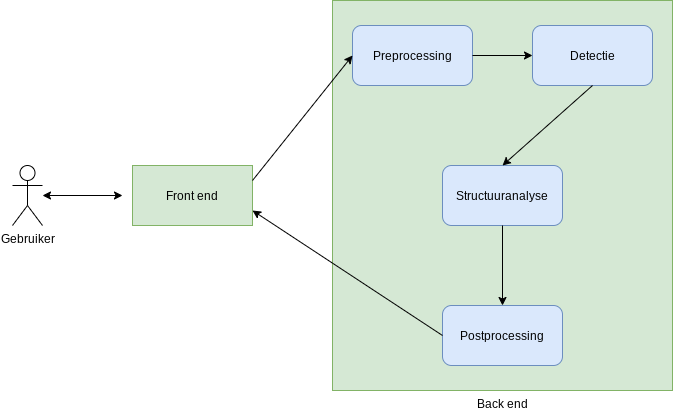
\includegraphics[width=1\textwidth]{img/proof_of_concept_architectuur.png}
    \caption{Architectuur van de proof-of-concept.}
    \label{fig:architectuur-proof-of-concept}
\end{figure}

In figuur \ref{fig:architectuur-proof-of-concept} wordt de architectuur van de proof-of-concept weergegeven, inclusief de verschillende componenten zoals \Gls{OCR}, tabeldetectie en meer. De datastroom, samen met de werking van de componenten, wordt in de volgende subsecties verder toegelicht.

\subsection{Documentinput}
\label{subsec:document-input}

Wanneer de gebruiker de software wil gebruiken, zal hij/zij een GUI zien die in de volgende figuur weergegeven wordt.

\begin{figure}[H]
    \centering
    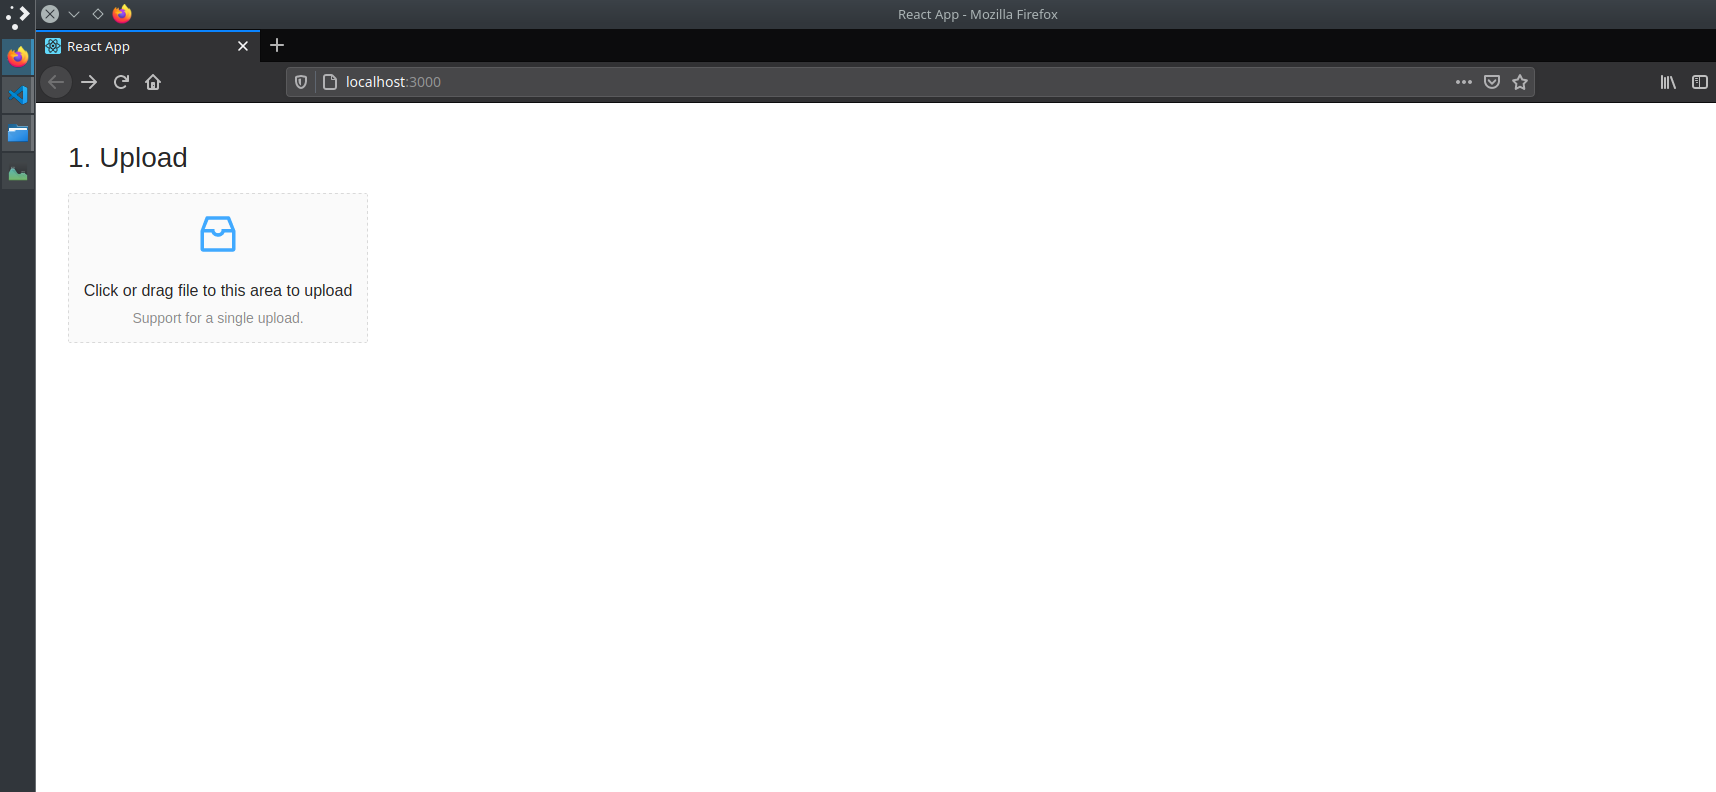
\includegraphics[width=1\textwidth]{img/gui_screenshot_not_used.png}
    \caption{GUI van de software bij eerste gebruik.}
    \label{fig:gui-screenshot-not-used}
\end{figure}

De gebruiker klikt op de upload-zone, waar de tekst ``Click or drag file to this area to upload`` vermeld staat. Vervolgens selecteert de gebruiker het document die getransformeerd moet worden. Bij de bevestiging van de selectie van het bestand wordt deze geüpload naar de back end, waar preprocessing plaatsvindt.

\subsection{Preprocessing}
\label{subsec:preprocessing}

Bij de preprocessing wordt extra witruimte toegevoegd aan de afbeelding. Dit is nodig omdat de tabeldetectiealgoritme, hoewel het zeer goed werkt op afbeeldingen van ingescande documenten, moeilijkheden heeft met tabeldetectie wanneer de afbeelding enkel uit de tabel zelf bestaat, zonder extra tekstelementen, witruimte, grafieken, figuren of dergelijke. Dit komt omdat de deep learning model getrained werd op documentafbeeldingen en niet op tabelafbeeldingen zelf. Eens de preprocessing uitgevoerd is, wordt tabeldetectie op de nieuwe afbeelding, waar extra witruimte aanwezig is, uitgevoerd.

\subsection{Tabeldetectie}
\label{subsec:tabel-detectie}

Voor de detectie wordt een drempel waarde (threshold) van 0,85 gekozen. Dit heeft als gevolg dat indien de berekende kans op de aanwezigheid van een tabel door de deep learning model gelijk is aan, of groter is dan 0,85, dan wordt de aanwezigheid van één of meerdere tabellen in de afbeelding als waar beschouwd; anders niet.

In onderstaande figuren \ref{fig:tabel-detectie-origineel} en \ref{fig:tabel-detectie-gedetecteerd} kan men respectievelijk links een origineel ingescande document zien en rechts de gedetecteerde tabellen in het document.

\begin{figure}[H]
    \centering
    \begin{minipage}{0.5\textwidth}
        \centering
        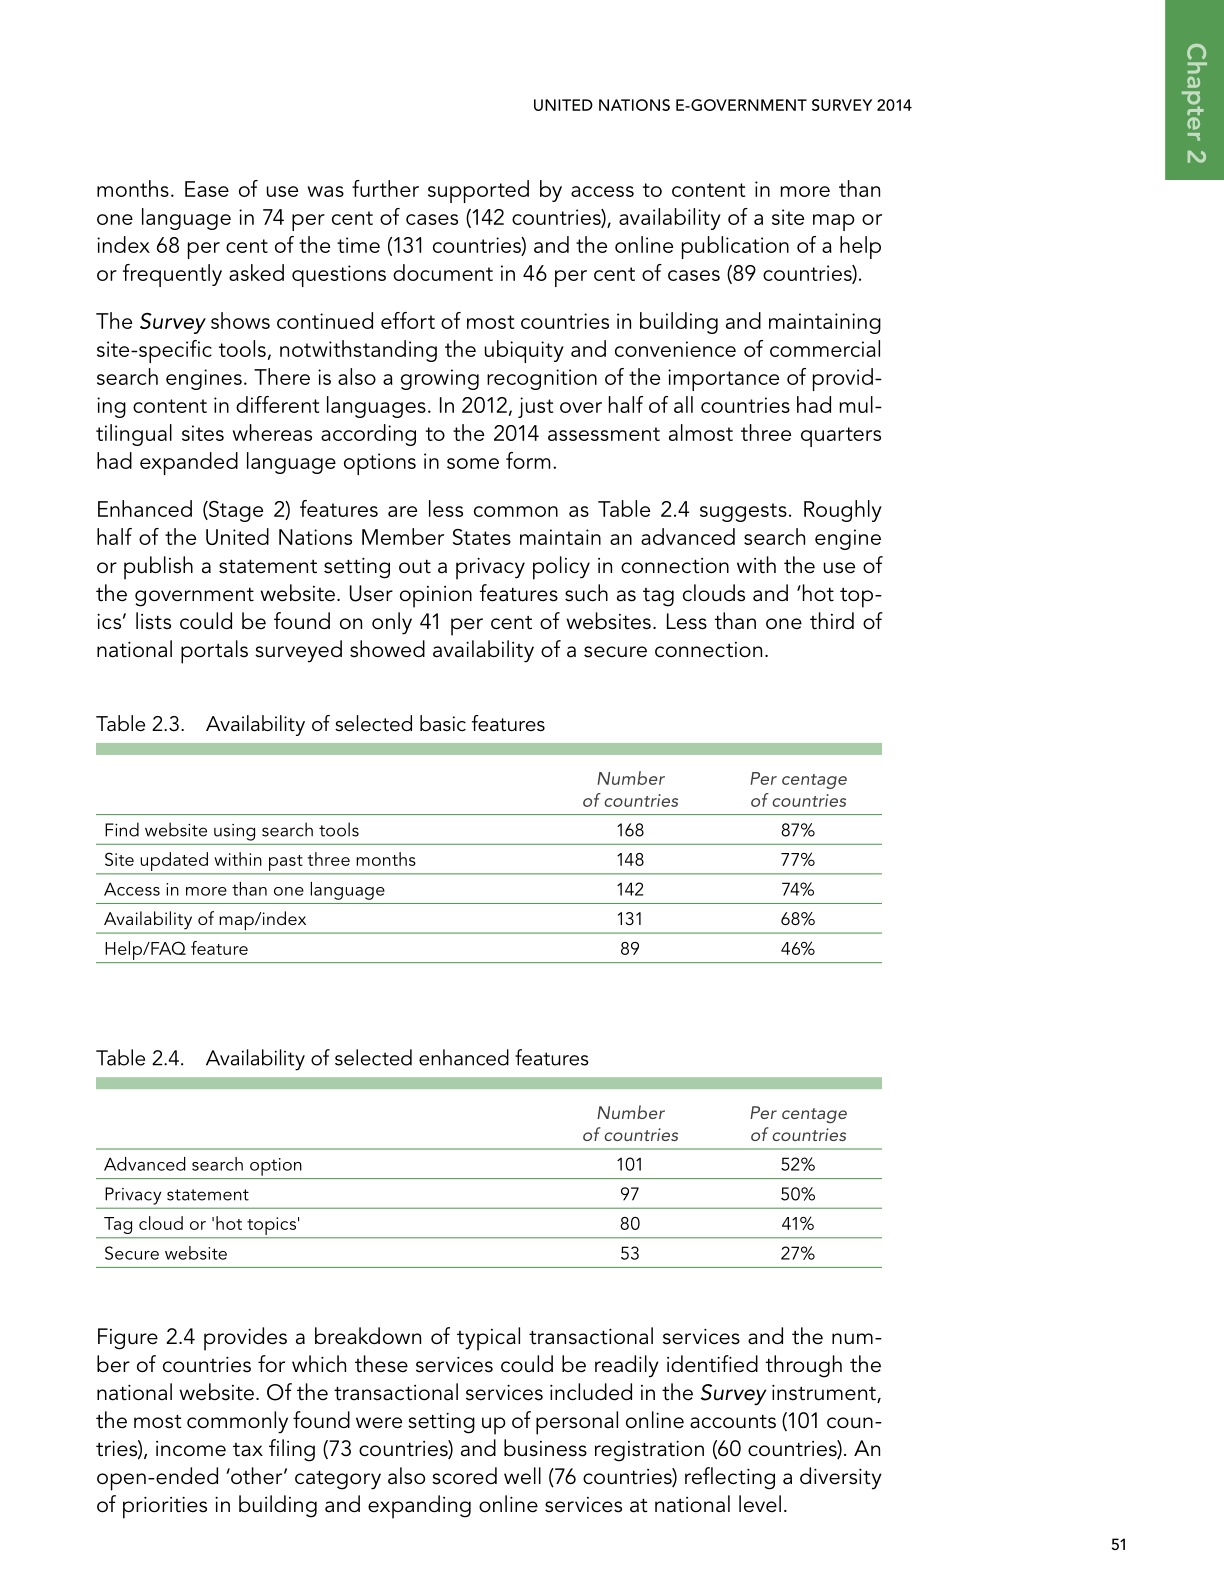
\includegraphics[width=1\textwidth]{img/tabel_detectie_voorbeeld_origineel.jpg}
        \caption{Origineel document}
        \label{fig:tabel-detectie-origineel}
    \end{minipage}\hfill
    \begin{minipage}{0.5\textwidth}
        \centering
        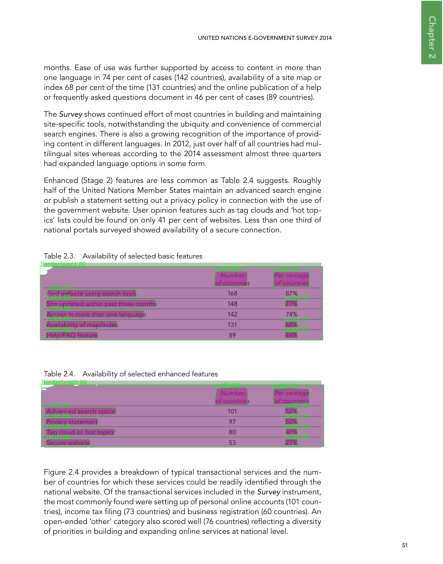
\includegraphics[width=1\textwidth]{img/tabel_detectie_voorbeeld_gedetecteerd.png}
        \caption{Gedetecteerde tabellen.}
        \label{fig:tabel-detectie-gedetecteerd}
    \end{minipage}
\end{figure}

Zoals men kan zien in figuur \ref{fig:tabel-detectie-gedetecteerd}, worden niet enkel de tabellen zelf maar eveneens cellen gedetecteerd. De detectie van tabellen is zeer accuraat, hoewel de detectie van cellen niet even nauwkeurig is. In de figuur bijvoorbeeld werden sommige cellen niet gedetecteerd.

Nadat de tabellen gedetecteerd zijn, worden ze bijgesneden om enkel de tabellen zelf te behouden en niet meer de rest van het document. Op elke geïsoleerd tabel worden de volgende stappen, tabelstructuuranalyse (\ref{subsec:tabel-structuur-analyse}) en postprocessing (\ref{subsec:post-processing}) uitgevoerd.

\subsection{Tabelstructuuranalyse}
\label{subsec:tabel-structuur-analyse}

\subsubsection{Origineel algoritme}
\label{subsubsec:origineel-algoritme}

Bij de tabelstructuuranalyse-algoritme van \textcite{Prasad2020}, die vanaf dit punt als ``algoritme A`` genoemd zal worden, wordt eerst gekeken naar de soort gedetecteerd tabel die bepaald en meegegeven werd door de tabeldetectie-component. Indien het om een bordered tabel gaat, wordt lijndetectie toegepast en wordt vervolgens d.m.v. cellsegmentatie aan elke cel een rij- en kolomwaarde toegekend. Anders, indien het dus als een borderless tabel gedetecteerd werd, wordt de positie van mogelijks gemiste, niet-gedetecteerde cellen voorspeld. De voorspelde cellen, samen met de reeds gedetecteerde cellen, worden vervolgens gebruikt om de rijen en kolommen te vormen.

Eens de tabel getransformeerd is, wordt het resultaat opgeslagen in een XML-bestand. Een voorbeeld hiervan wordt in de volgende code \ref{lst:xml-resultaat} weergegeven.\newpage

\lstinputlisting[language=XML, caption={Voorbeeld van een XML-resultaat-bestand.}, captionpos=b, label={lst:xml-resultaat}]{code/resultaat_tabelstructuuranalyse_voorbeeld.xml}

Daaropvolgend wordt de XML-resultaat-bestand geïtereerd. Bij een ``cell``-XML-tag wordt gekeken naar de coördinaten en dimensies (gespecifieerd door de ``Coords``-XML-tag van de ``cell``-tag) en op basis hiervan wordt \Gls{OCR} op enkel die regio toegepast. Hierdoor verkrijgt men de tekst te vinden binnen de celregio, gedefinieerd door de XML-resultaat. Dit proces wordt iteratief uitgevoerd op elke ``cell``-tag. Door middel van de tekst en rij- en kolomwaarden (gespecifieerd door respectievelijk de ``start/end-row``- en ``start/end-col``-attribuut) van elke cel wordt tenslotte een Pandas Dataframe aangemaakt die de getransformeerd tabel bevat.

\subsubsection{Voorgesteld verbeterd algoritme}
\label{subsubsec:origineel-algoritme}

In tabelafbeeldingen waarin voldoende ruimte aanwezig is tussen de cellen (in geval van borderless tabellen) of in tabelafbeeldingen waarin de horizontale en verticale scheidingslijnen goed te onderscheiden zijn van de rest van de tabel (in geval van bordered tabellen), is algoritme A bruikbaar. Echter, zoals reeds aangegeven, worden de cellen door de tabeldetectiemodel niet altijd gedetecteerd. Ook zijn tabelscheidingslijnen soms moeilijk te onderscheiden van andere lijnen, zoals de lijnen die gevormd worden door letters zoals de `l` of `p`. Door deze complicaties werkt algoritme A meestal niet.

Daarom worden enkele aanpassingen voorgesteld voor de tabelstructuuranalyse, die gezamenlijk als ``algoritme B`` genoemd zullen worden.

Voor bordered tabellen wordt een verbetering van de lijndetectie-algoritme voorgesteld.

De verschillende stappen die genomen worden bij lijndetectie worden gedemonstreerd d.m.v. de volgende figuur \ref{fig:lijn-detectie-origineel}.

\begin{figure}[H]
    \centering
    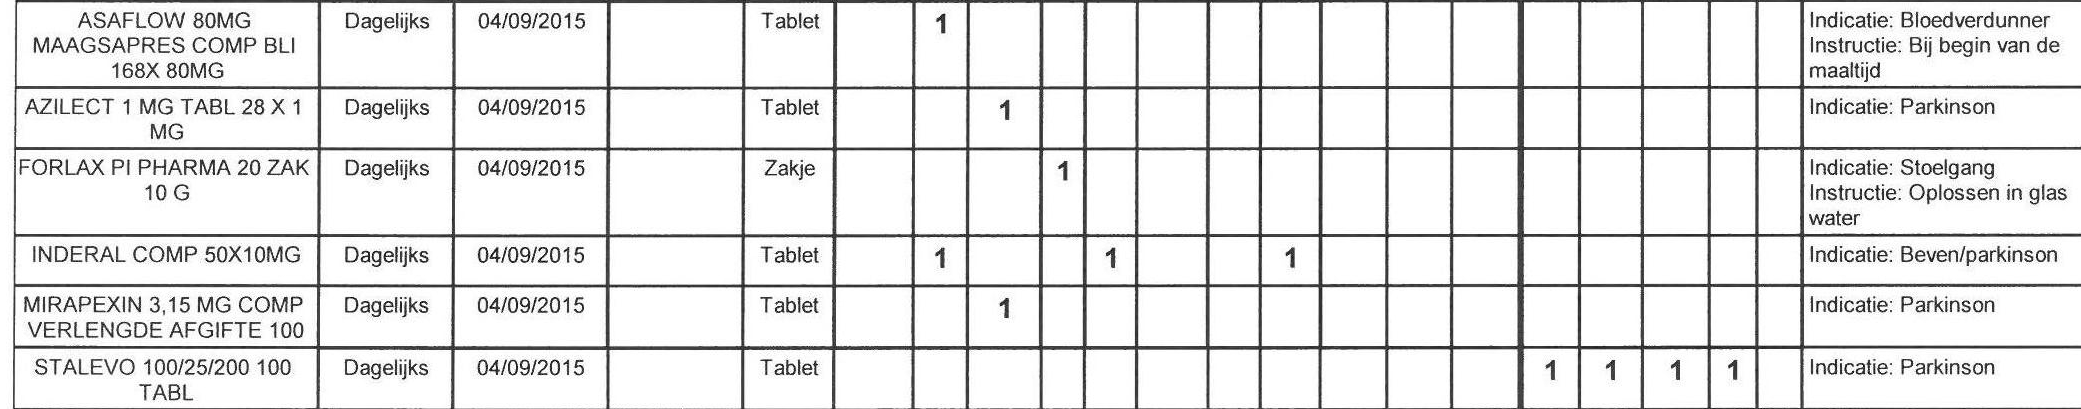
\includegraphics[width=1\textwidth]{img/lijn_detectie_origineel.png}
    \caption{Origineel geïsoleerd tabel.}
    \label{fig:lijn-detectie-origineel}
\end{figure}

In algoritme A, om de horizontale en verticale scheidingslijnen van de tabel te detecteren, wordt in een eerste stap, adaptive thresholding toegepast. Bij simpele thresholding wordt een afbeelding in kleur gesegmenteerd, meestal tot een zwart-wit-versie van de afbeelding. Indien de intensiteit van een pixel, bij simpele thresholding, een vaste threshold (drempelwaarde) overschrijdt, wordt de pixel als zwart gesegmenteerd, anders als wit. Bij adaptive thresholding is de waarde van de threshold afhankelijk van de regio waarin de pixel zich bevindt. In de volgende figuur werd adaptive thresholding toegepast op de origineel figuur \ref{fig:lijn-detectie-origineel}.

\begin{figure}[H]
    \centering
    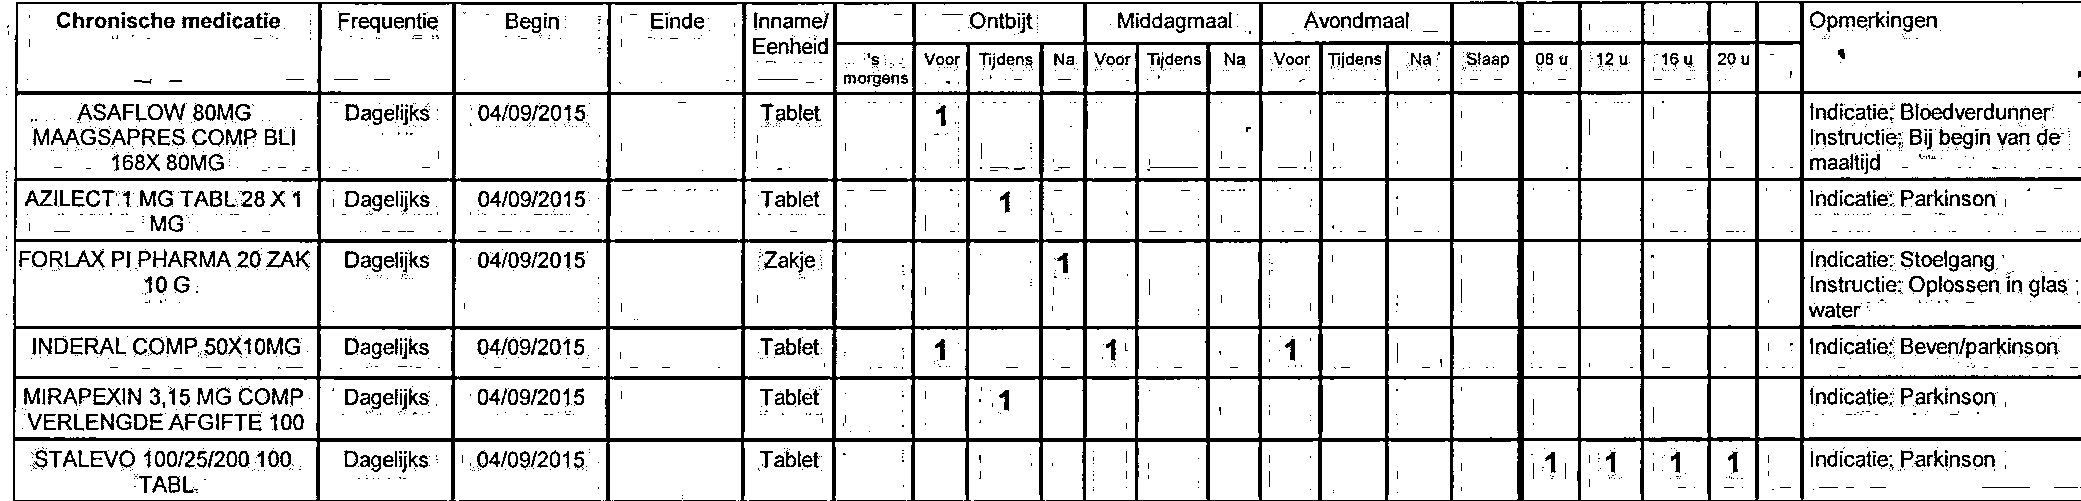
\includegraphics[width=1\textwidth]{img/line_detection_a_1_adaptive_threshold_on_image.png}
    \caption{Adaptive thresholding.}
\end{figure}

Vervolgens wordt een bitwise-not-operatie uitgevoerd. Dit heeft als gevolg dat de kleuren geïnverteerd worden.

\begin{figure}[H]
    \centering
    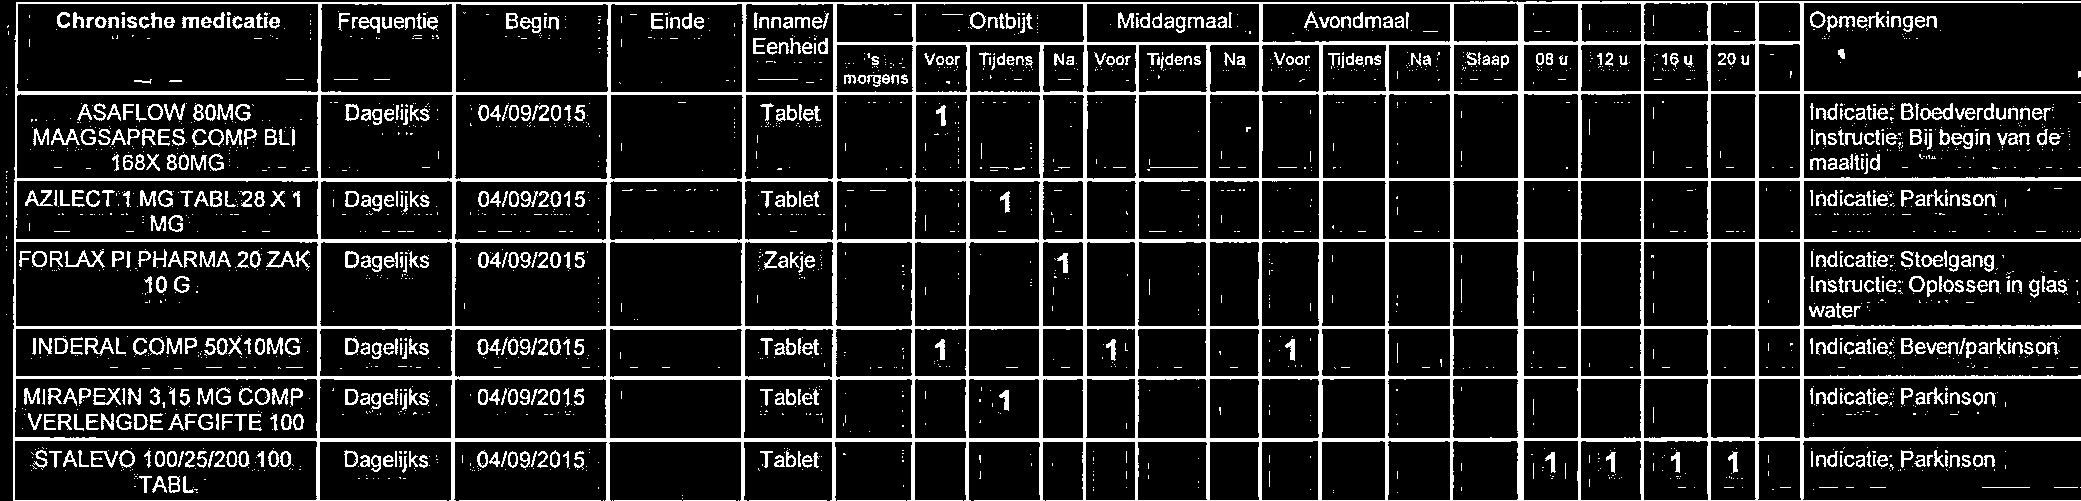
\includegraphics[width=1\textwidth]{img/line_detection_a_2_bitwise_not_on_image.png}
    \caption{Bitwise-not-operatie.}
\end{figure}

Hierna, om horizontale lijnen te detecteren, worden de pixels geërodeerd d.m.v. een horizontale structuur.

\begin{figure}[H]
    \centering
    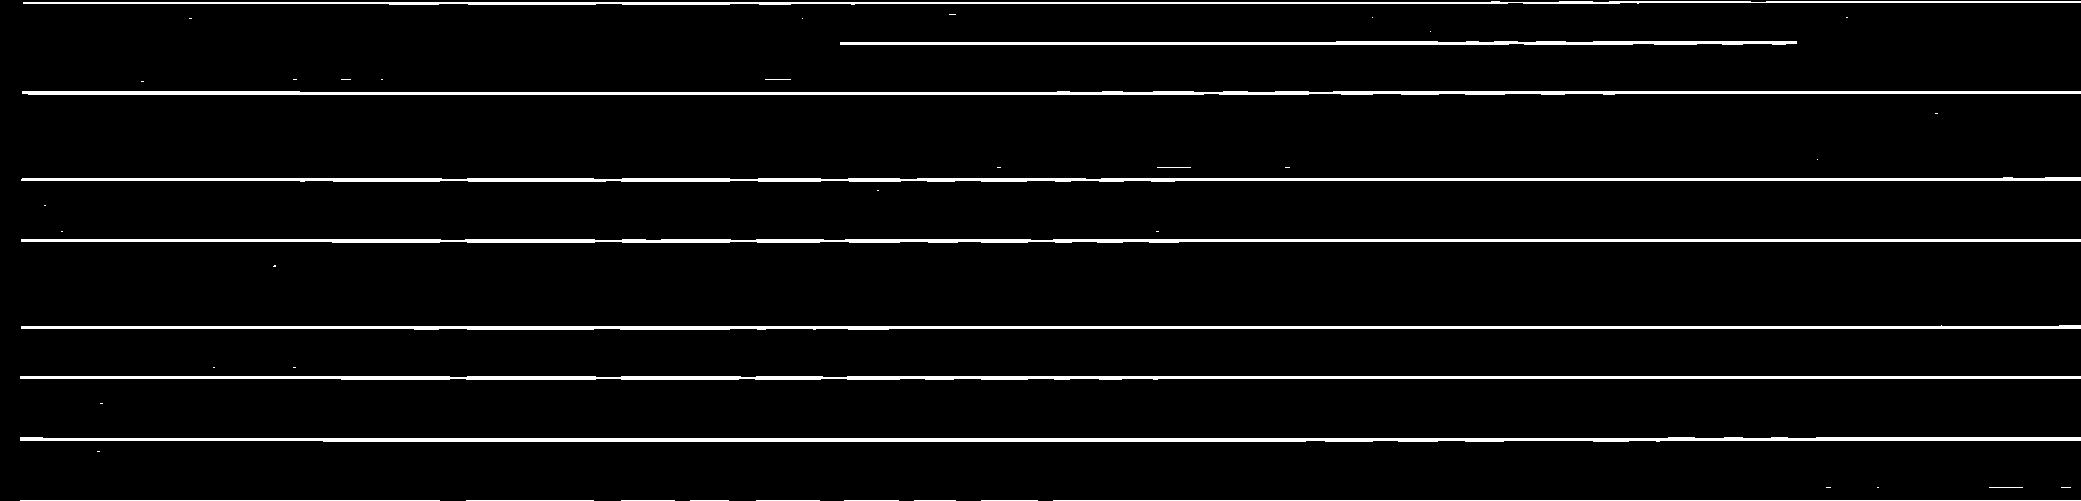
\includegraphics[width=1\textwidth]{img/line_detection_a_3_erode_horizontal_structure_for_horizontal_lines.png}
    \caption{Erosie d.m.v. een horizontale structuur.}
\end{figure}

Nadien vindt een dilatatie van de pixels plaats, d.m.v. de horizontale structuur.

\begin{figure}[H]
    \centering
    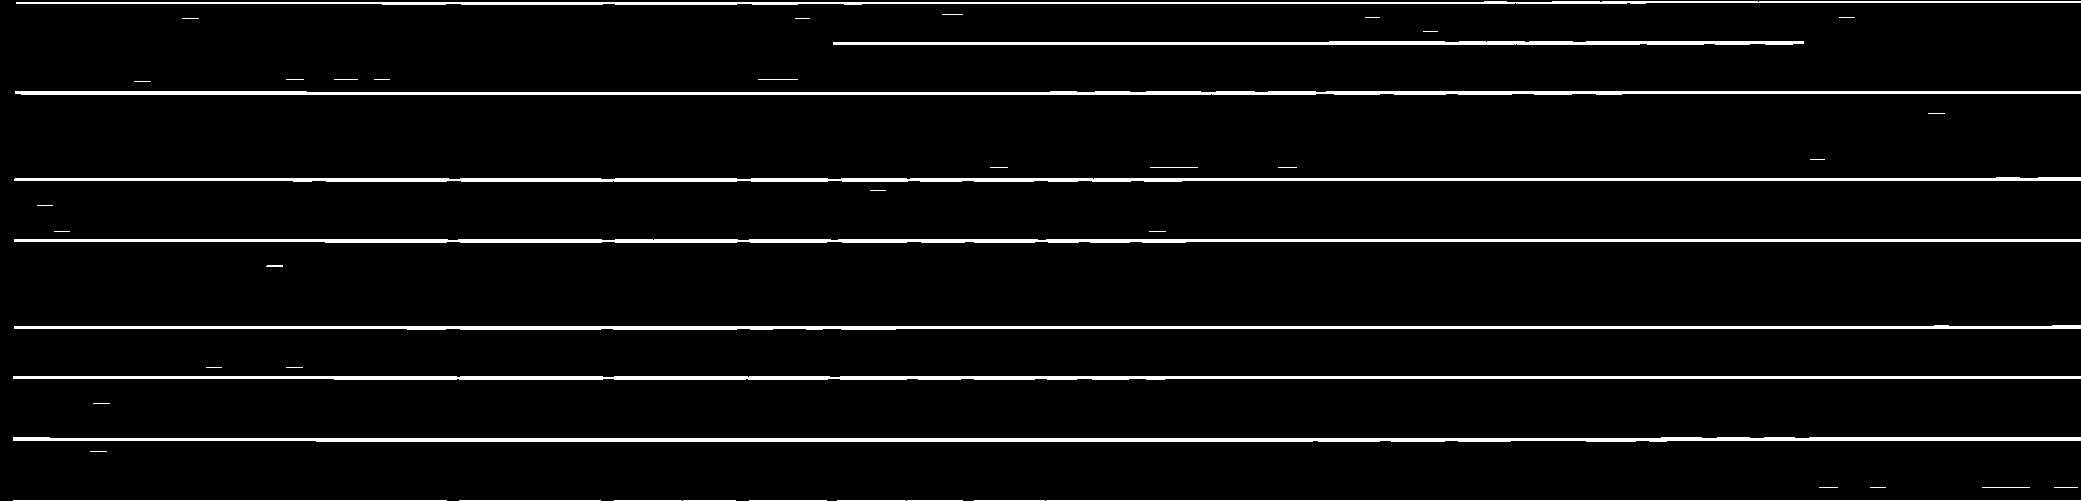
\includegraphics[width=1\textwidth]{img/line_detection_a_4_dilate_horizontal_structure_for_horizontal_lines.png}
    \caption{Dilatatie d.m.v. de horizontale structuur.}
\end{figure}

Hierna wordt een simpele dilatatie uitgevoerd, gevolgd door een simpele erosie.

\begin{figure}[H]
    \centering
    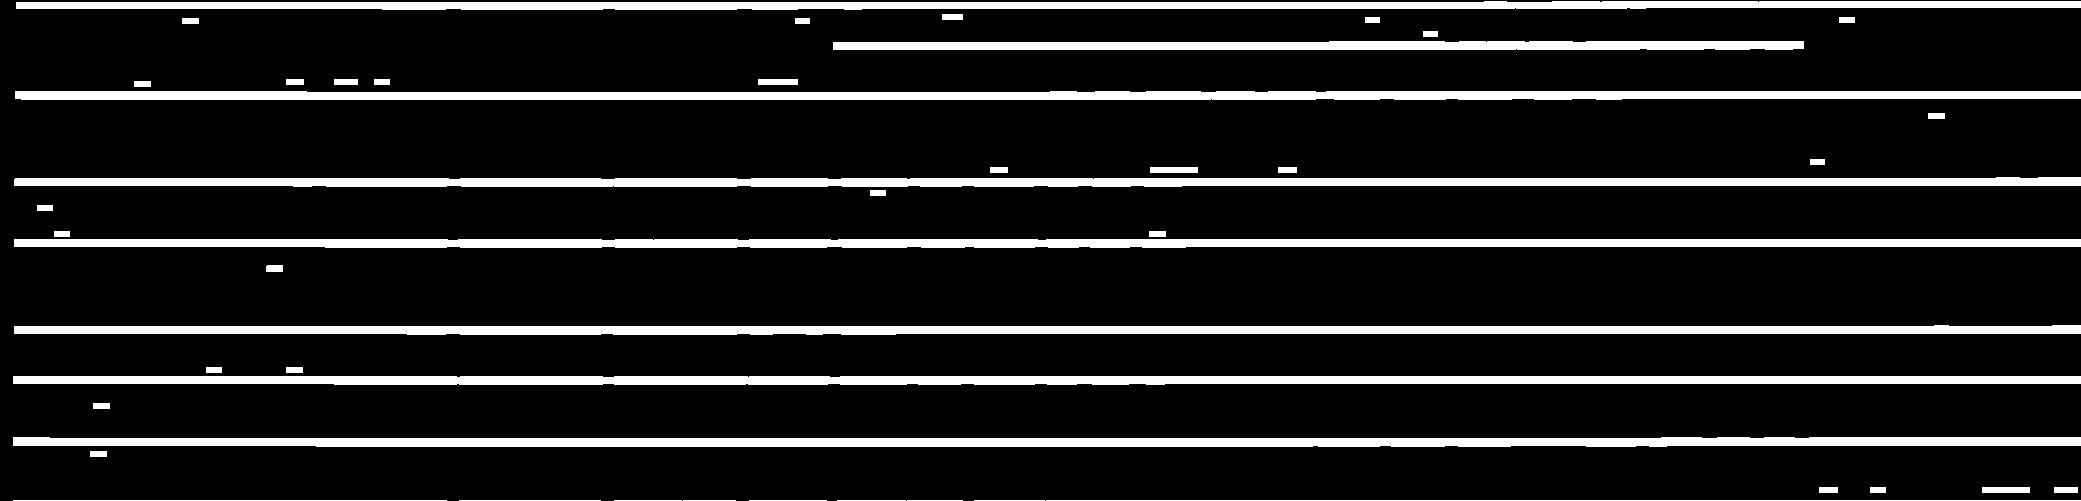
\includegraphics[width=1\textwidth]{img/line_detection_a_5_dilate_image_for_horizontal_lines.png}
    \caption{Simpele dilatatie.}
\end{figure}

\begin{figure}[H]
    \centering
    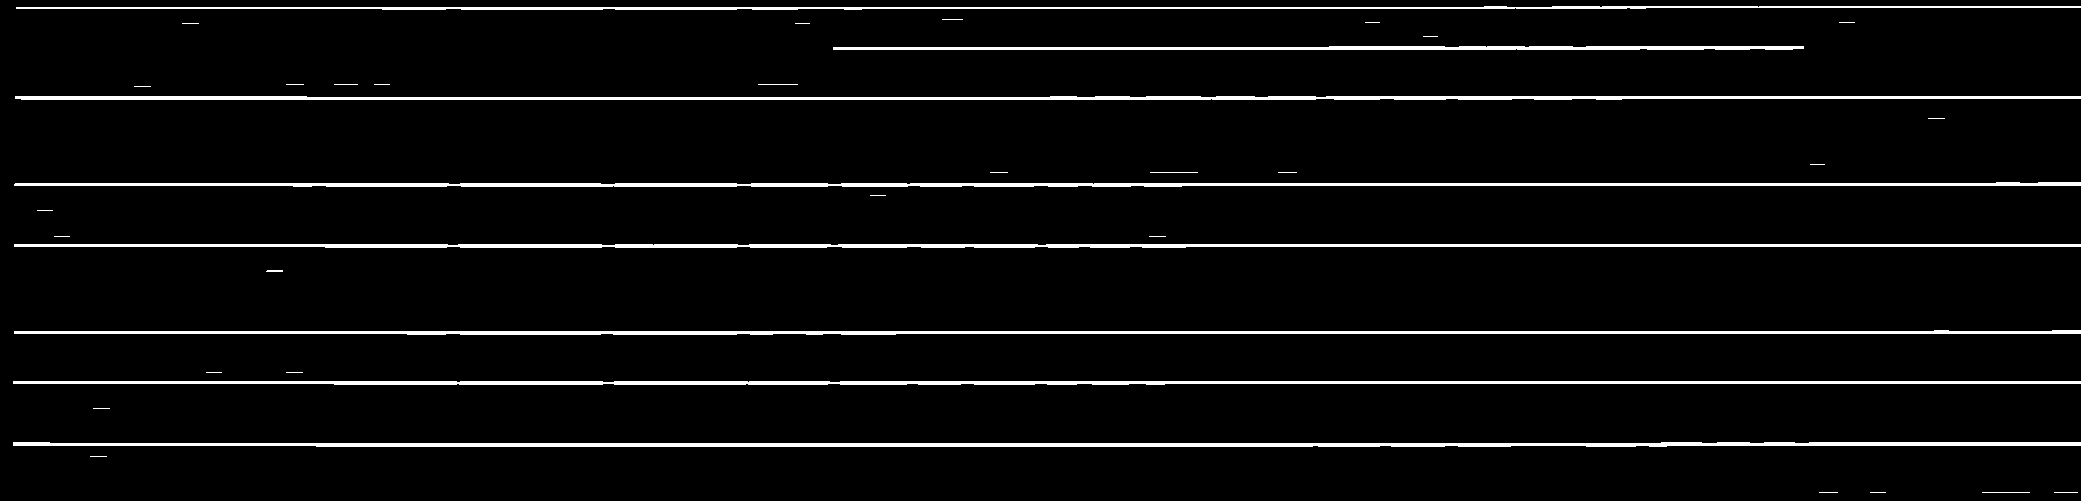
\includegraphics[width=1\textwidth]{img/line_detection_a_6_erode_image_for_horizontal_lines.png}
    \caption{Simpele erosie.}
\end{figure}

Uiteindelijk worden horizontale structuren met een te kleine lengte buiten beschouwing gebracht en wordt een Hough Line-transformatie uitgevoerd. Zo worden de horizontale lijnen verkregen. Op een analoog manier worden de verticale lijnen gedetecteerd. De gedetecteerde lijnen zijn in figuur \ref{fig:lines-detected-a} in rood en groen voorgesteld.

\begin{figure}[H]
    \centering
    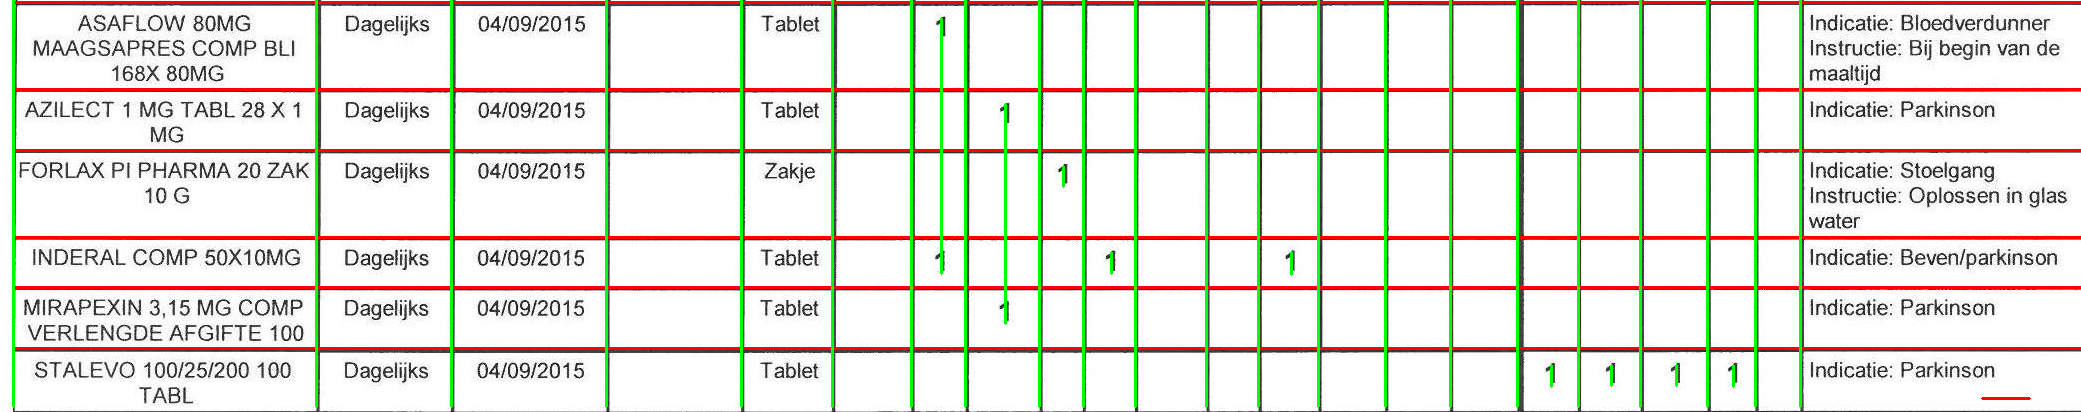
\includegraphics[width=1\textwidth]{img/lines_detected_a.png}
    \caption{Lijnen gedetecteerd door algoritme A.}
    \label{fig:lines-detected-a}
\end{figure}

Met algoritme B wordt een andere aanpak voor de lijnendetectie voorgesteld.

Zo worden eerst de tekstblokken, gedetecteerd door \Gls{OCR}, gemaskeerd door witte rechthoeken om de tekstelementen binnen de tabel te verbergen. In de volgende figuur \ref{fig:line-detection-b-text-removed} wordt het resultaat van deze operatie weergegeven. Men kan merken dat er nog tekstelementen aanwezig zijn. Dit komt omdat de resolutie van de ingescande document laag is, waardoor de \Gls{OCR}-software niet alle tekstblokken heeft kunnen detecteren.

\begin{figure}[H]
    \centering
    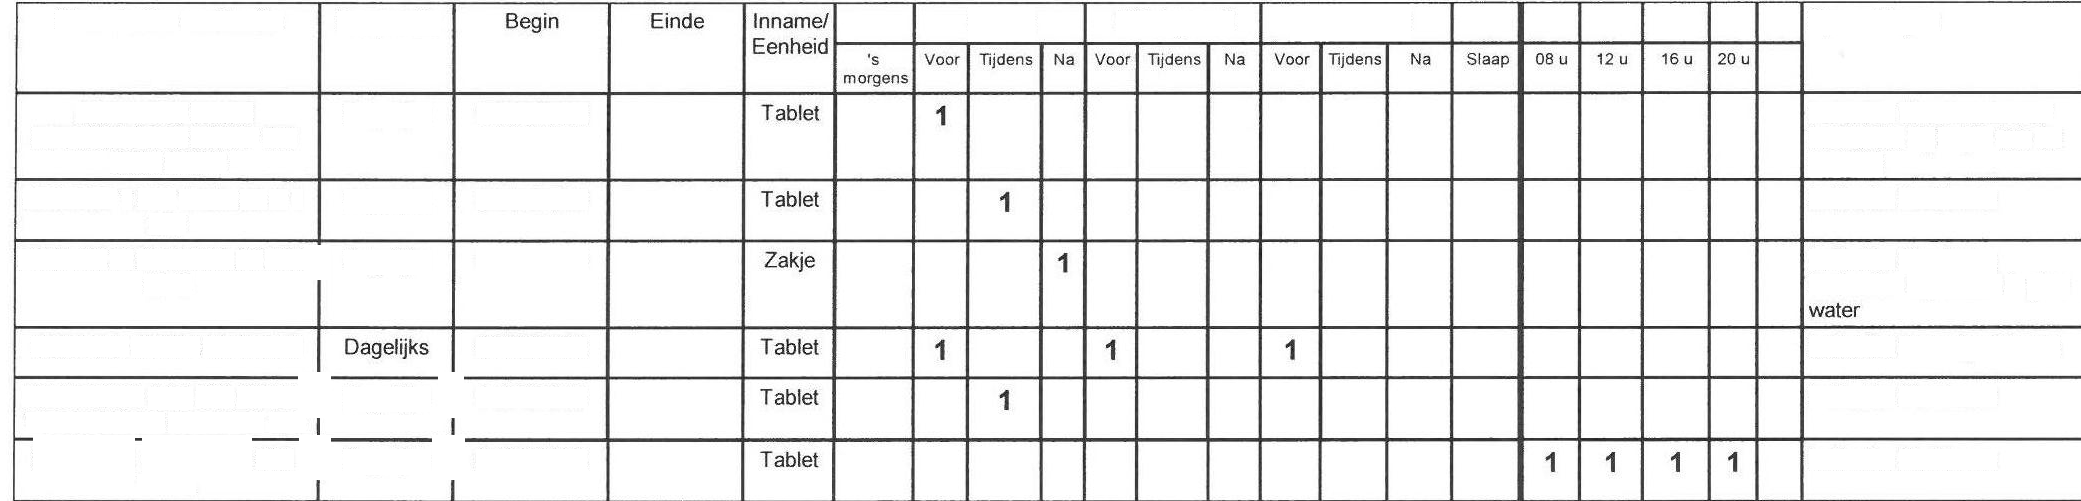
\includegraphics[width=1\textwidth]{img/line_detection_b_1_detected_text_removed.png}
    \caption{Verwijdering van tekstelementen.}
    \label{fig:line-detection-b-text-removed}
\end{figure}

Vervolgens wordt een dilatatie, gevolgd door een erosie uitgevoerd.

\begin{figure}[H]
    \centering
    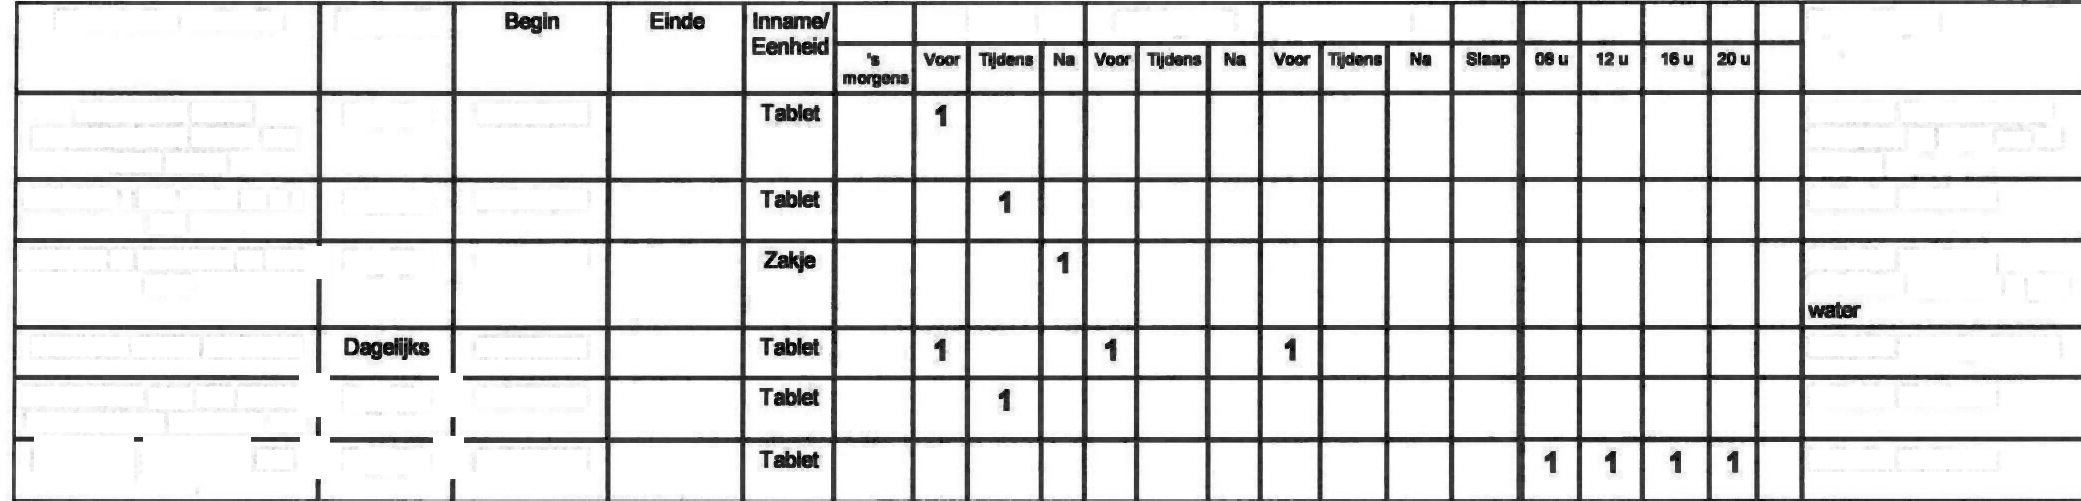
\includegraphics[width=1\textwidth]{img/line_detection_b_2_image_eroded.png}
    \caption{Dilatatie.}
\end{figure}

\begin{figure}[H]
    \centering
    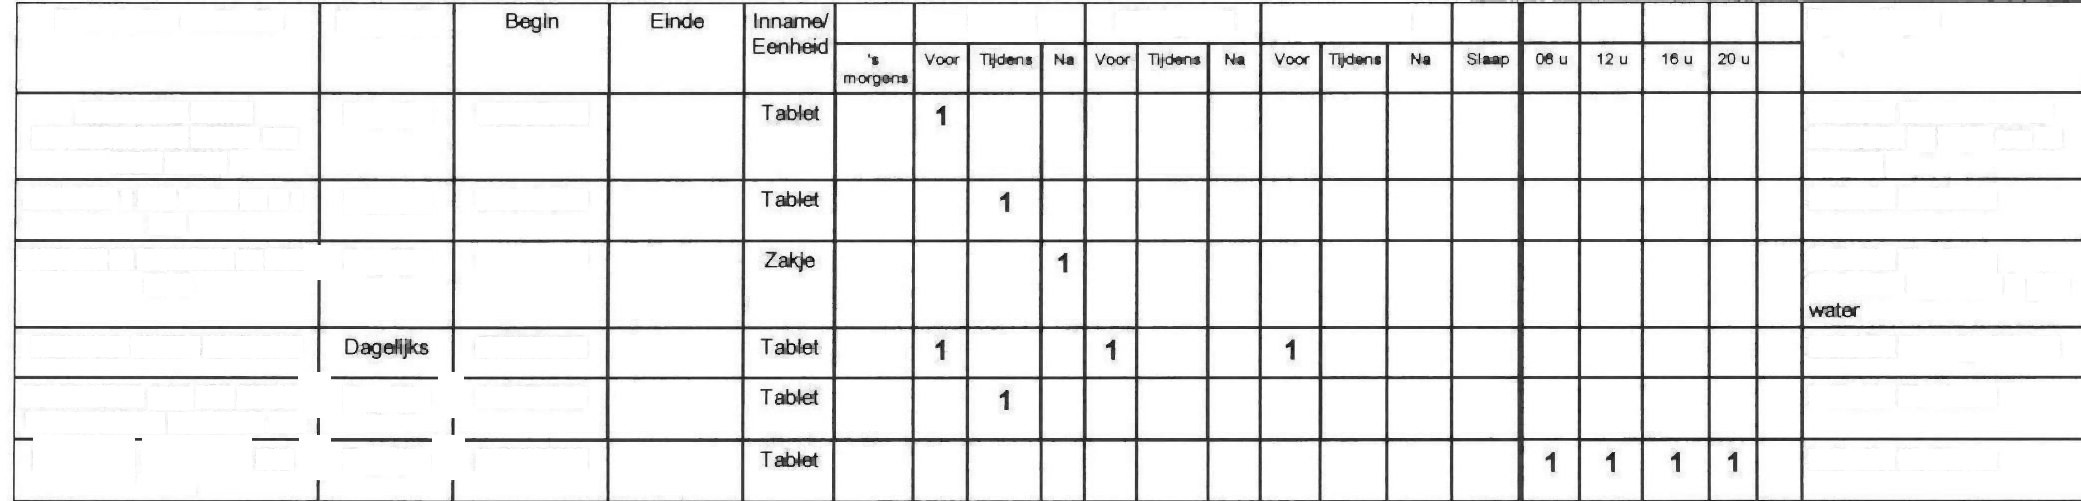
\includegraphics[width=1\textwidth]{img/line_detection_b_3_image_dilated.png}
    \caption{Erosie.}
\end{figure}

Uiteindelijk worden een Canny edge-operatie en een Hough-Line-transformatie toegepast om de horizontale en verticale tegelijk te detecteren. Deze gedetecteerde lijnen zijn in figuur \ref{fig:lines-detected-b} in rood en groen voorgesteld.

\begin{figure}[H]
    \centering
    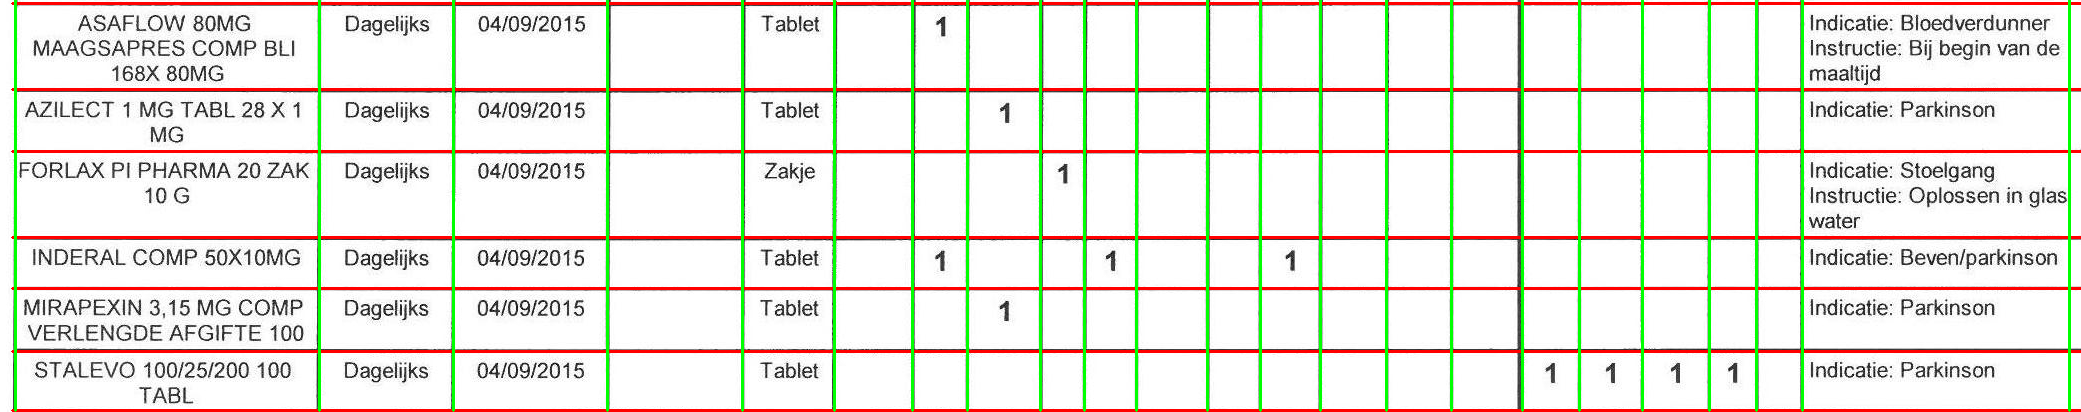
\includegraphics[width=1\textwidth]{img/lines_detected_b.png}
    \caption{Lijnen gedetecteerd door algoritme B.}
    \label{fig:lines-detected-b}
\end{figure}

Met de volgende figuren \ref{fig:lines-detected-a} en \ref{fig:lines-detected-b} wordt het resultaat van beide algoritmes opnieuw weergegeven.

\begin{figure}[H]
    \centering
    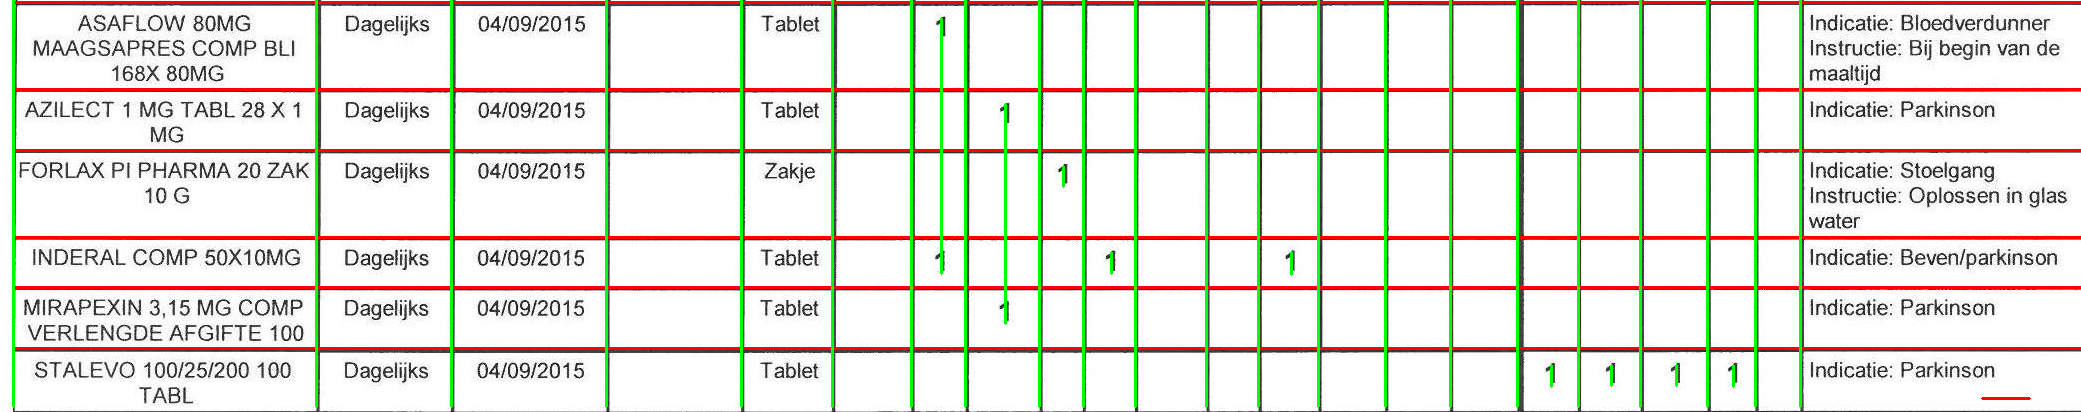
\includegraphics[width=1\textwidth]{img/lines_detected_a.png}
    \caption{Lijnen gedetecteerd door algoritme A.}
    \label{fig:lines-detected-a-overzicht}
\end{figure}

\begin{figure}[H]
    \centering
    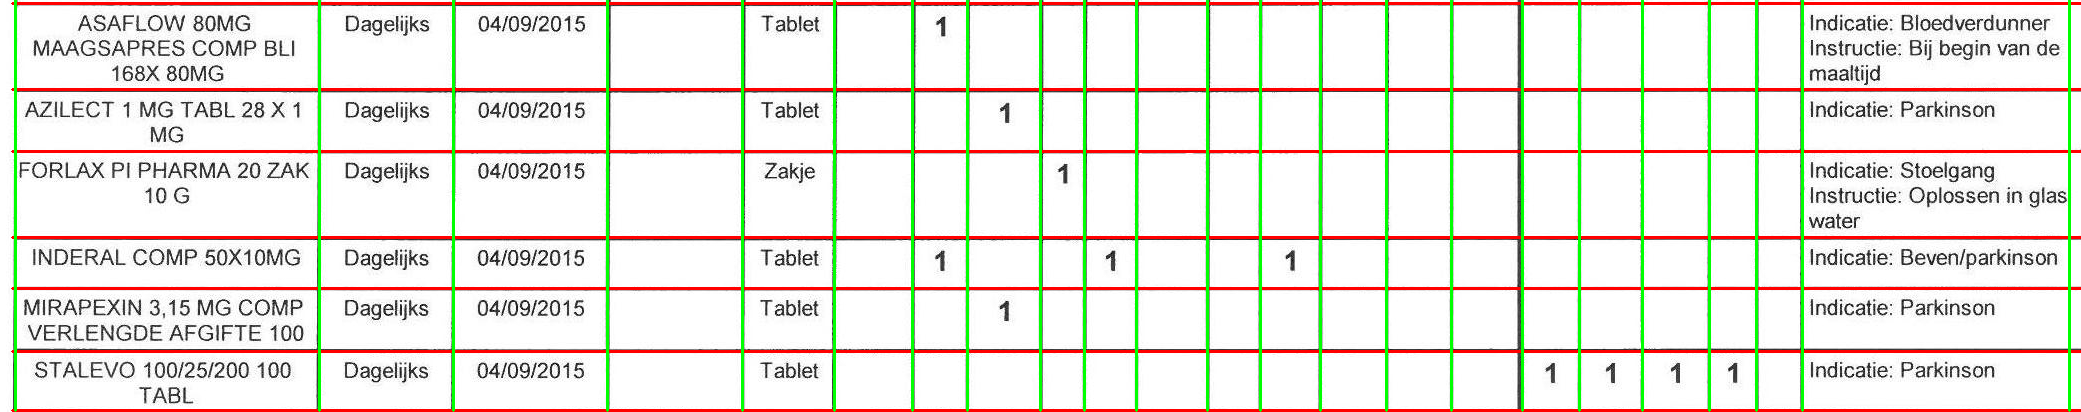
\includegraphics[width=1\textwidth]{img/lines_detected_b.png}
    \caption{Lijnen gedetecteerd door algoritme B.}
    \label{fig:lines-detected-b-overzicht}
\end{figure}

Zoals men kan zien, heeft algoritme A last van valse positieven. Er worden namelijk teveel lijnen gedetecteerd. Dit komt enerzijds omdat het de streep van de tekstelementen ``1`` als verticale lijnen detecteerd. Anderzijds wordt door afbeeldingruis een extra horizontaal lijn, rechts onderaan, gedetecteerd. Met algoritme B worden alle lijnen correct gedetecteerd.

Voor borderless tabellen wordt een clusteringalgoritme voorgesteld, in combinatie met lijndetectie. Bij borderless tabellen kan men een bepaalde patroon herkennen. Het verschil in X-positie tussen tekstblokken van verschillende kolommen is namelijk veel groter dan het verschil in X-positie tussen tekstblokken binnen dezelfde kolom. Overeenkomstig is het verschil in Y-positie tussen tekstblokken van verschillende rijden veel groter dan het verschil in Y-positie tussen tekstblokken binnen dezelfde rij. Dit betekent dat men cellen kan clusteren (groeperen) op basis van hun X-Y-positie in rij- en kolomclusters. Deze rij- en kolomclusters worden in relatie gebracht met bepaalde rij- en kolomindexen. Zo kan men door clustering aan elk cel een rij- en kolomindex toekennen. Een populair clusteringalgoritme is K-means-clustering. Echter moet hiervoor het aantal clusters meegegeven worden, wat niet mogelijk is aangezien het aantal rijen en kolommen van een willekeurig tabel niet op voorhand gekend is. Daarom wordt voor Algoritme B, voor de clustering van cellen van borderless tabellen, gebruikgemaakt van hiërarchische clustering die op basis van een maximum afstand werkt.

\subsection{Postprocessing}
\label{subsec:post-processing}

Aangezien algoritme B op \Gls{OCR} steunt voor tabelstructuuranalyse, is een postprocessing van het resultaat noodzakelijk. Postprocessing is niet nodig indien gebruik gemaakt wordt van algoritme A.

Eens een Pandas Dataframe, met daarin tekstelementen met bijhorende rij- en kolomwaarden, verkregen is d.m.v. algoritme B, vindt concatenatie plaats. Hierbij worden tekstblokken die dezelfde rij- en kolomwaarden hebben, aan elkaar geconcateneerd. Bovendien worden volledige lege rijen en kolommen verwijderd van de Pandas Dataframe.

\subsection{Resultaatweergave}
\label{subsec:resultaat-weergave}

Na de strucuuranalyse, en postprocessing indien algoritme A gebruikt werd, wordt de Pandas Dataframe omgezet in een JSON-object die teruggestuurd wordt van de back end naar de GUI van de gebruiker. De gebruiker krijgt dan het resultaat van de tabeltransformatie te zien.

\begin{figure}[H]
    \centering
    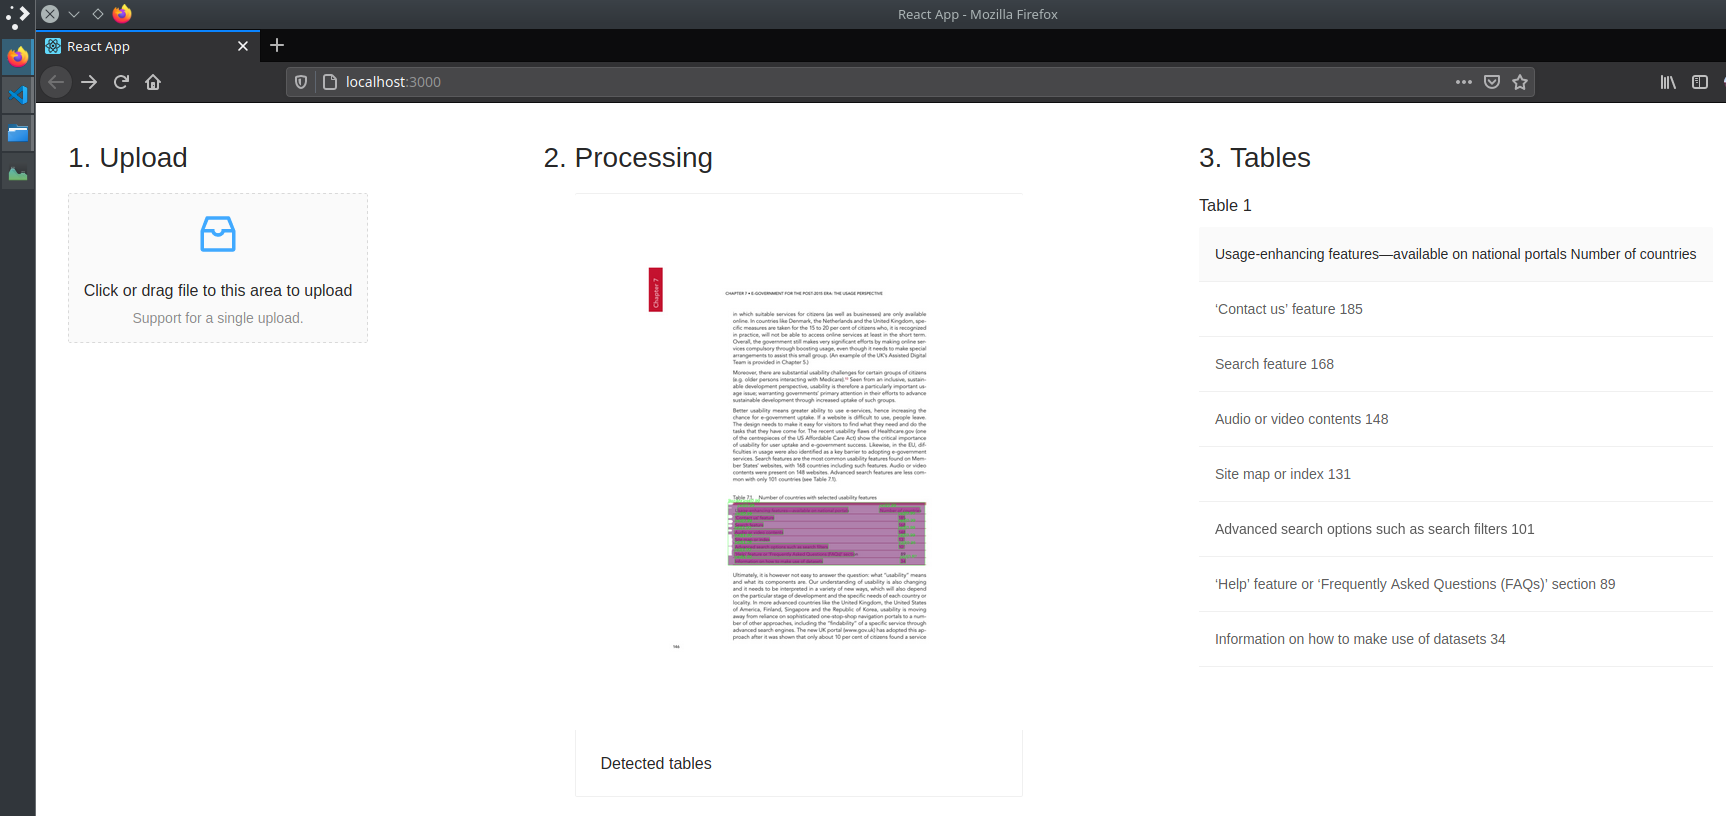
\includegraphics[width=1\textwidth]{img/gui_screenshot_used.png}
    \caption{GUI van de software wanneer de tabeltransformatie uitgevoerd is.}
    \label{fig:gui-screenshot-used}
\end{figure}

\section{Praktisch gebruik}
\label{sec:praktisch-gebruik}

\subsection{Hardware- en software-vereisten}
\label{subsec:hardware-en-software-vereisten}

Wat hardware betreft, is een grafische kaart van het merk NVIDIA nodig. Dit komt omdat, voor de tabeldetectie, \textcite{Prasad2020} gebruik maakt van een verouderd versie van MMDetection \autocite{Chen2019}, een objectdetectie-library. Bij de meest recente versie van MMDetection is objectdetectie d.m.v. enkel de CPU mogelijk. 

Wat software betreft is een Linux-distributie of MacOS nodig voor de tabeldetectie, aangezien MMDetection niet ondersteund wordt op het besturingssysteem Windows. Indien de tabellen reeds geïsoleerd zijn en dus enkel tabelstructuuranalyse nodig is, dan is tabeldetectie niet nodig en kan de software eveneens op Windows gebruikt worden.

\subsection{Installatie en gebruik}
\label{subsec:installatie-en-gebruik}

De open source broncode, inclusief gedetailleerde installatie- en gebruiksinstructies zijn te vinden in de repository \textcite{Nazari2020}.
